%%%%%%%%%%%%%%%%%%%%%%%%%%%%%%%%%%%%%%%%%
% Professional Newsletter Template
% LaTeX Template
% Version 1.0 (09/03/14)
%
% Created by:
% Bob Kerstetter (https://www.tug.org/texshowcase/) and extensively modified by:
% Vel (vel@latextemplates.com)
% 
% This template has been downloaded from:
% http://www.LaTeXTemplates.com
%
% License:
% CC BY-NC-SA 3.0 (http://creativecommons.org/licenses/by-nc-sa/3.0/)
%
%%%%%%%%%%%%%%%%%%%%%%%%%%%%%%%%%%%%%%%%%

\documentclass[9pt]{extarticle} % The default font size is 10pt; 11pt and 12pt are alternatives

%%%%%%%%%%%%%%%%%%%%%%%%%%%%%%%%%%%%%%%%%
% Professional Newsletter Template
% Structural Definitions File
% Version 1.0 (09/03/14)
%
% Created by:
% Vel (vel@latextemplates.com)
% 
% This file has been downloaded from:
% http://www.LaTeXTemplates.com
%
% License:
% CC BY-NC-SA 3.0 (http://creativecommons.org/licenses/by-nc-sa/3.0/)
%
%%%%%%%%%%%%%%%%%%%%%%%%%%%%%%%%%%%%%%%%%

%----------------------------------------------------------------------------------------
%	REQUIRED PACKAGES
%----------------------------------------------------------------------------------------

\usepackage{listings}
\usepackage{graphicx} % Required for including images
\usepackage{microtype} % Improved typography
\usepackage{multicol} % Used for the two-column layout of the document
\usepackage{booktabs} % Required for nice horizontal rules in tables
\usepackage{wrapfig} % Required for in-line images
\usepackage{float} % Required for forcing figures not to float with the [H] parameter
\usepackage[utf8]{inputenc}
\usepackage{fancyhdr}

%------------------------------------------------
% Fonts

\usepackage{charter} % Use the Charter font as the main document font
\usepackage{courier} % Use the Courier font for \texttt (monospaced) only
\usepackage[T1]{fontenc} % Use T1 font encoding

%------------------------------------------------
% List Separation

\usepackage{enumitem} % Required to customize the list environments
\setlist{noitemsep,nolistsep} % Remove spacing before, after and within lists for a compact look

%------------------------------------------------
% Figure and Table Caption Styles

\usepackage{caption} % Required for changing caption styles
\captionsetup[table]{labelfont={bf,sf},labelsep=period,justification=justified} % Specify the table caption style
\captionsetup[figure]{labelfont={sf,bf},labelsep=period,justification=justified, font=small} % Specify the figure caption style
\setlength{\abovecaptionskip}{10pt} % Whitespace above captions

%------------------------------------------------
% Spacing Between Paragraphs

\makeatletter
\usepackage{parskip}
\setlength{\parskip}{6pt}
\newcommand{\@minipagerestore}{\setlength{\parskip}{6pt}}
\makeatother

%----------------------------------------------------------------------------------------
%	PAGE MARGINS AND SPACINGS
%----------------------------------------------------------------------------------------

\textwidth = 7 in % Text width
\textheight = 10 in % Text height
\oddsidemargin = -18pt % Left side margin on odd pages
\evensidemargin = -18pt % Left side margin on even pages
\topmargin = -36pt % Top margin
\headheight = 0pt % Remove the header by setting its space to 0
\headsep = 0pt % Remove the space between the header and top of the page
\parskip = 2pt % Space between paragraph
\parindent = 0.0in % Paragraph indentation
\pagestyle{empty} % Disable page numbering

%----------------------------------------------------------------------------------------
%	COLORS
%----------------------------------------------------------------------------------------

\usepackage[dvipsnames,svgnames]{xcolor} % Required to specify custom colors

\definecolor{altncolor}{rgb}{.8,0,0} % Dark red
%\definecolor{altncolor}{rgb}{.2,.4,.8} % Dark blue
%\definecolor{altncolor}{rgb}{.84,.16,.16} % Red

\usepackage[colorlinks=true, linkcolor=altncolor, anchorcolor=altncolor, citecolor=altncolor, filecolor=altncolor, menucolor=altncolor, urlcolor=altncolor]{hyperref} % Use the color defined above for all links

%----------------------------------------------------------------------------------------
%	BOX STYLES
%----------------------------------------------------------------------------------------

\usepackage[framemethod=TikZ]{mdframed}% Required for creating boxes
\mdfdefinestyle{sidebar}{
    linecolor=black, % Outer line color
    outerlinewidth=0.5pt, % Outer line width
    roundcorner=0pt, % Amount of corner rounding
    innertopmargin=10pt, % Top margin
    innerbottommargin=10pt, % Bottom margin
    innerrightmargin=10pt, % Right margin
    innerleftmargin=10pt, % Left margin
    backgroundcolor=white, % Box background color
    frametitlebackgroundcolor=white, % Title background color
    frametitlerule=false, % Title rule - true or false
    frametitlerulecolor=white, % Title rule color
    frametitlerulewidth=0.5pt, % Title rule width
    frametitlefont=\Large, % Title heading font specification
    font=\small
}

\mdfdefinestyle{intextbox}{
    linecolor=black, % Outer line color
    outerlinewidth=0.5pt, % Outer line width
    roundcorner=10pt, % Amount of corner rounding
    innertopmargin=7pt, % Top margin
    innerbottommargin=7pt, % Bottom margin
    innerrightmargin=7pt, % Right margin
    innerleftmargin=7pt, % Left margin
    backgroundcolor=white, % Box background color
    frametitlebackgroundcolor=white, % Title background color
    frametitlerule=false, % Title rule - true or false
    frametitlerulecolor=white, % Title rule color
    frametitlerulewidth=0.5pt, % Title rule width
    frametitlefont=\Large % Title heading font specification
}

%----------------------------------------------------------------------------------------
%	HEADING STYLE
%----------------------------------------------------------------------------------------

\newcommand{\heading}[2]{ % Define the \heading command
\vspace{#2} % White space above the heading
{\begin{center}\Large\textbf{#1}\end{center}} % The heading style
\vspace{#2} % White space below the heading
}

\newcommand{\BackToContents}{\hyperlink{contents}{{\small Back to Contents}}} % Define a command for linking back to the contents of the newsletter % Include the document which specifies all packages and structural customizations for this template

\begin{document}

%--------------------------------------------------------------------------------
% HEADER DETAILS
%--------------------------------------------------------------------------------

\pagestyle{fancy}
\fancyhf{}
\chead{segfault@csh.rit.edu}
\rhead{\today}
\lhead{Volume XLVI Issue \#{3}}
\addtolength\footskip{-15px}
\cfoot{"I don't want my sister on Cohoe." ~Ethan House (ehouse)}

%----------------------------------------------------------------------------------------
%	HEADER IMAGE
%----------------------------------------------------------------------------------------

\begin{figure}[H]
\centering\vspace{0.5cm}
\includegraphics[width=0.8\linewidth]{segfault.png}
\end{figure}

%--------------------------------------------------------------------------------
% HEADER QUOTE
%--------------------------------------------------------------------------------

\vspace{-15px}
\begin{quote}
\centering
\textbf{\textit{"Random chance seems to have operated in our favor"}}
\end{quote}
\vspace{10px}

%----------------------------------------------------------------------------------------
%	SIDEBAR - FIRST PAGE
%----------------------------------------------------------------------------------------

\vspace{-0.5cm}\begin{minipage}[t]{.30\linewidth} % Mini page taking up 30% of the actual page
\begin{mdframed}[style=sidebar,frametitle={}] % Sidebar box

%-----------------------------------------------------------

\hypertarget{contents}{\textbf{{\large This week on floor\ldots}}} % \hypertarget provides a label to reference using \hyperlink{label}{link text}
\begin{itemize}
\item \hyperlink{firstnews}{Imagine RIT}
\item \hyperlink{secondnews}{ret = brk()}
\item \hyperlink{thirdnews}{User Comic: git init --bear}
\end{itemize}

\centerline {\rule{.75\linewidth}{.25pt}} % Horizontal line

%-----------------------------------------------------------

\textbf{Notable Upcoming Events:}
\begin{enumerate}[leftmargin=0.5cm]
\item \textbf{Accepted Student Open House} @ April 4th
\item \textbf{Photo Hunt} @ April 18th
\item \textbf{War Paint Challenge} @ March 6th
\end{enumerate}

%-----------------------------------------------------------

\textbf{Googlers Everywhere}

Technically active, semi-alumnus, but really demigod member Russ Harmon (russ) dropped by floor this week as part of a Google recruiting drive. Russ's efforts to educate and push floor members has earned him quite the reputation among active members and alumni alike. Joining him at Google will be current History director Josh McSavaney (mcsaucy), and co-op'ing at Google this semester will be member Drew Gottlieb (dag10).

\textbf{Call to Pay Dues}

If you have not payed dues this semester, please do so by contacting current Financial directory Derek Gonyeo (dgonyeo). If dues are not paid, you will not be able to vote in elections, house votes, or any other director meeting. \textbf{If you cannot pay dues for financial reasons or otherwise, please let the financial directory know.} CSH is dedicated to using it's funds for its members.

\textbf{Selections Committee Coming Up}

Evaluations Director Tal Cohen (tcohen) would like to remind active members that the time for selections committee is nearing. As mentioned in previous articles, the selections committee is in charge of evaluating new applications to CSH, and will be working with Housing to sort applicants.

%-----------------------------------------------------------

\captionof*{table}{Voting Results}
\begin{tabular}{lcr}

Vote & Cost & Result \\
\midrule
\bottomrule
\end{tabular}

%-----------------------------------------------------------

\end{mdframed}
\end{minipage}\hfill % End the sidebar mini page 
%
%----------------------------------------------------------------------------------------
%	MAIN BODY - FIRST PAGE
%----------------------------------------------------------------------------------------
%
\begin{minipage}[t]{.66\linewidth} % Mini page taking up 66% of the actual page
\vspace{-0.4cm}
\hypertarget{firstnews}{\heading{Imagine RIT}{6pt}}

Officially, Imagine RIT is an annual event hosted on campus that is open to the public, and generally attracts people to see student works. An excerpt from RIT's website says:

\begin{quote}
Imagine RIT is designed to demonstrate what can be accomplished when, as RIT President Bill Destler likes to say, “the right and left brain collide.” Visitors have witnessed a robot that serves hot dogs, a concrete canoe that floats and dozens of musical and theatrical performances. Children have made freeze-dried ice cream, test driven Segways and jumped around in a bounce house.
\end{quote}

This kind of human interaction has traditionally let students garner some attention for their neat projects, and has inspired many to seek funding or academic support. CSH has participated for several years, and often gathers quite the crowd at our unique booths. A call submissions to Imagine RIT has been out for a while, and if you'd like to have your project featured in the festival, talk to the Research \& Development Director Travis Whitaker (tmobile).

%-----------------------------------------------------------

\hypertarget{secondnews}{\heading{ret = brk()}{6pt}} 

This editor, like many editors previous, would like some Member content for the weekly publication. The content genre isn't so important, so long as the quality is at least worth a cursory readover. In particular this editor would appreciate posts regarding user environments, (programming) language preferences, philophical arguments regarding technology, and as an aside, haikus. To have at least one "real-world" technically relevant section per publication would be ideal.

Floor Directors, this editor would particularly like your input for upcoming events that may or may not have made it to Webnews. Votes that have occurred are not tracked through any central system, making it difficult to find relevant outcomes.

Responses, comments, complaints, or corrections should go to segfault@csh.rit.edu.
\textit{Particularly radical submissions may be awarded a mysterious token of the value \$2.56, from the bank of Segfault}

\hypertarget{thirdnews}{\heading{User Comic: git init --bear}{6pt}} 

\begin{center}
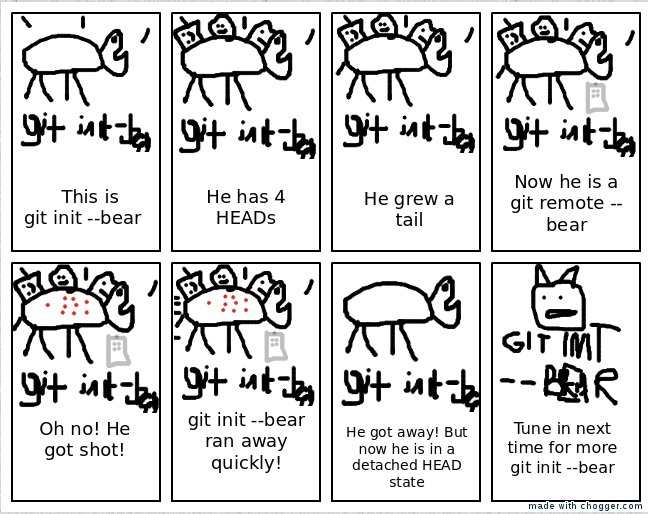
\includegraphics[scale=0.40]{git_init_comic.png}
\end{center}

\end{minipage} % End the main body - first page mini page

\end{document} 